\documentclass[twoside,11pt]{article}

% Any additional packages needed should be included after jmlr2e.
% Note that jmlr2e.sty includes epsfig, amssymb, natbib and graphicx,
% and defines many common macros, such as 'proof' and 'example'.
%
% It also sets the bibliographystyle to plainnat; for more information on
% natbib citation styles, see the natbib documentation, a copy of which
% is archived at http://www.jmlr.org/format/natbib.pdf

\usepackage{jmlr2e}
\usepackage{graphicx}
\graphicspath{{./}}

% Definitions of handy macros can go here

\newcommand{\dataset}{{\cal D}}
\newcommand{\fracpartial}[2]{\frac{\partial #1}{\partial  #2}}
\newcommand{\code}[1]{\texttt{#1}}
\newcommand{\titleofpaper}{Conformer-RL}
% Heading arguments are {volume}{year}{pages}{date submitted}{date published}{paper id}{author-full-names}

% TODO: update heading
% \jmlrheading{volume}{year}{pages}{date submitted}{date published}{paper id}{Jiang et al.}

% Short headings should be running head and authors last names
\ShortHeadings{\titleofpaper}{Jiang et al.}
\firstpageno{1}

\begin{document}

\title{\titleofpaper}

% TODO: update authors
\author{\name Runxuan Jiang \email runxuanj@umich.edu \\
       \name Tarun Gogineni \email tgog@umich.edu \\
       \name Joshua Kammeraad \email joshkamm@umich.edu\\
       \name Ambuj Tewari \email tewaria@umich.edu\\
       \name Paul Zimmerman \email paulzim@umich.edu\\
       \addr
       University of Michigan\\
       Ann Arbor, MI 48109, USA} 
% TODO: update editors
\editor{TBD}

\maketitle

\begin{abstract}%   <- trailing '%' for backward compatibility of .sty file
  We present \code{\titleofpaper}, an open-source deep reinforcement learning library designed for molecular conformer generation using Python. The library contains modular interfaces for environments and agents, allowing users to easily build and test new implementations. Also included are several pre-built pre-built environments and agents based on state-of-the-art algorithms in the field to serve as baselines. Additionally, \code{\titleofpaper} comes with extensive logging and visualization tools for evaluation of agents and generated conformers, as well as a toolkit for generating and modifying molecules. \code{\titleofpaper} is well-tested and thoroughly documented, and is available through on PyPi and on Github: \code{https://github.com/ZimmermanGroup/conformer-ml}.
\end{abstract}

\begin{keywords}
  reinforcement learning, deep learning, deep reinforcement learning, open source, conformer generation, computational chemistry
\end{keywords}

\section{Introduction}
Recently, much progress has been made in the application of deep reinforcement learning to tasks in computational chemistry \citep{li2018foldingzero,zhou2017reactions,simm2020moldesign}. One task where deep reinforcement learning showed promising results is conformer generation \citep{gogineni2020torsionnet}, which involves finding an ensemble of unique low-energy three-dimensional orientations, or conformers, for a given molecule \citep{ebejer2020confgen}. Efficient and accurate prediction of low-energy conformers is integral to molecular modeling, with wide applications from drug development to 3D QSAR \citep{cole2018confgen}. However, there currently exists very few open-source software libraries for deep reinforcement learning applied conformer generation, and the ones that do exist are often not modular enough for further experimentation and modification. To address this issue, we introduce \code{\titleofpaper}, a comprehensive and modular Python library for applying deep reinforcement learning to conformer generation, using PyTorch \citep{torch} for deep learning and RDKit for chemoinformatic capabilities.

Many libraries already exist that contain benchmarking experiments and baseline implementations for general deep reinforcement learning. For example, OpenAI Gym \citep{brockman2016gym} and bsuite \citep{osband2020bsuite} both contain implementations of reinforcement learning environments commonly used for benchmarking agents, such as cartpole, mountaincar, and Atari. \code{\titleofpaper} seeks to fill this role within the conformer generation space by supplying pre-built environments for benchmarking agents. Additionally, \code{\titleofpaper} includes an environment interface to easily customize environments for further exploration. This allows \code{\titleofpaper}'s environment to be readily modified for other chemoinformatic tasks related to conformer generation, such as protein folding and reaction prediction.

There are also many implementations of baseline deep reinforcement learning agents available, such as Rllib \citep{liang2018rllib} and OpenAI baselines \citep{dhariwal2018baselines}. However, due to the complex nature of molecules which are often represented by graph structures rather than vectors, a large amount of modification and setup work is required to adapt these baseline libraries to work with molecule environments. Within \code{\titleofpaper}, we include a general agent base class for building agents compatible with conformer generation environments, as well as several baseline reinforcement learning algorithms. Also included are baseline implementations neural network architectures for molecule inputs built with graph neural network (GNN) components using PyTorch Geometric \citep{fey2019geometric}.

Additionally, \code{\titleofpaper} provides extensive logging capabilities and an analysis module for recording and visualizing training results, including conformer-generation specific metrics and visuals.

\section{\titleofpaper Architecture}
\begin{figure}[h]
  \centering
  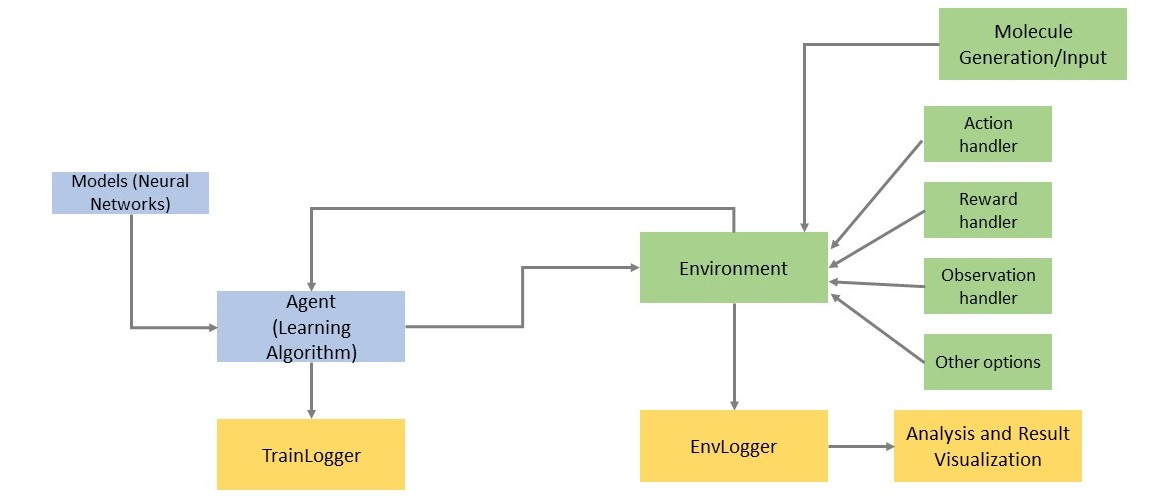
\includegraphics[width=\textwidth]{architectures.jpg}
  \caption{Architecture of \code{\titleofpaper}. Agent components are colored blue, environment components are colored green, and logging/analysis componenets are colored yellow.}
  \label{fig:architecture}
\end{figure}
  A visual representation of the architecture can be seen in figure \ref{fig:architecture}.

\subsection{Environments}
\code{\titleofpaper} environments are classes built on top of the \code{ConformerEnv} base class. The methods in \code{ConformerEnv} are implemented in a way so that each method corresponds to a different component within the environment, and is independent to the behavior of the other components. The main components include:
\begin{itemize}
  \item \textbf{Action Handler} is implemented by overriding the \code{\_step(action)} method. The action handler determines how the environment processes an incoming action. Usually this corresponds to generating a new conformer based on the action.
  \item \textbf{Reward Handler} is implemented by overriding the \code{\_reward()} method. The reward handler returns a reward based on the current state of the environment.
  \item \textbf{Observation Handler} is implemented by overriding the \code{\_obs()} method. The observation handler returns an observation object based on the current state of the environment and is a compatible input for the neural network of the agent.
\end{itemize}
Other class methods of \code{ConformerEnv} can also be overridden at the user's convenience. For example, if the user would like to keep track of the number of conformers generated with an energy below a certain threshold for each episode, they may add a member variable \code{self.confs\_below\_threshold = 0} to the \code{reset()} method, and then update \code{self.confs\_below\_threshold} within the action handler.

For each environment component, \code{\titleofpaper} implements several pre-built options in the form of mixin classes. Due to the flexibility of the design of \code{ConformerEnv}, different handlers can be mixed and matched to form unique environments, and new environments for tasks related to conformer generation, such as protein folding, can be easily built by implementing custom versions of the components.

\code{\titleofpaper} also includes wrappers for executing multiple environments in parallel. 

  \subsubsection{Molecule Generation}
  \code{\titleofpaper} environments are designed to configurable with different molecules, including user-generated ones. Environments are initizlied with a \code{MolConfig} object, which specifies the RDKit molecule to be used in the environment and any molecule-specific parameters.

  For convenience, \code{\titleofpaper} contains scripts for generating \code{MolConfig} objects for several simple molecules and molecule benchmarks found in \citet{gogineni2020torsionnet}, such as branched alkanes, lignin, and more.

\subsection{Agents and Models}
Agents in \code{\titleofpaper} are classes inheriting from the \code{BaseAgent} base class. Agents are initialized with a \code{Config} object, which specifies the neural network model to be used, training environment, optimize function, and other hyperparameters. Agents can also be configured with an evaluation environment, in which the agent will only evaluate on but not train on. The base class also handles logging. Custom agents can be created by overriding the \code{step()} method of \code{BaseAgent}, which corresponds to one iteration of interacting with the environment to collect samples and then training on those samples.

\code{\titleofpaper} implements several baseline built-in agents, including recurrent and non-recurrent implementations of advantage actor critic (A2C) \citep{wu2017a2c} and proximal policy optimization (PPO) \citep{schulman2017ppo}.

\code{\titleofpaper} implements several baseline built-in neural network models, including recurrent and non-recurrent versions of the \code{\titleofpaper} model from \citep{gogineni2020torsionnet} which utilizes a message passing neural network (MPNN) \citep{gilmer2017mpnn}, as well as similar graph networks that utilize graph attention networks \citep{gatnn}.

\subsection{Logging and Analysis}
The \code{\titleofpaper} library contains two types of loggers:
\begin{itemize}
  \item \code{TrainLogger} is designed to record information from the agent during training, such as (but not limited to) total reward per episode, training loss, runtime, and memory used. \code{TrainLogger} supports logging data directly to TensorBoard \citep{tensorflow2015-whitepaper}, where the data can be visualized in real time and downloaded if needed.
  \item \code{EnvLogger} is designed to record environment information across a single episode, such as (but not limited to) the conformers generated, and the energy of each generated conformer. \code{EnvLogger} supports saving the per-episode data as a \code{.pickle} file, as well as saving each generated molecule conformer separately as a \code{.mol} file. The saved files can then be loaded into a notebook and visualized by \code{\titleofpaper}'s analysis toolkit.
\end{itemize}
Both loggers are integrated into the \code{BaseAgent} and \code{ConformerEnv} interfaces, and are readily accessible when writing new agents or environments.

\code{\titleofpaper} contains an analysis toolkit for calculating conformer-related metrics and visualizing results. The toolkit is designed to be used in a notebook and uses seaborn \citep{waskom2021seaborn} to generate figures and molecule visualization tools to generate interactive three-dimensional visuals for molecule conformers.

\section{Usage and Documentation}
\code{\titleofpaper} provides a detailed API reference for all functions, classes, and non-private class methods in the library. We also provide eight example scripts for training pre-built agents on pre-built environments, and a jupyter notebook showing example usage of the analysis toolkit on logged data. The quick start section of the documentation covers how to run the training scripts, switch between prebuilt environments and agents, and tuning hyperparameters. Finally, we provide a guide on how to build a custom environment from scratch, and train an agent on the environment.

\section{Conclusion}
\code{\titleofpaper} is a comprehensive library with tools for each step of the pipeline for training and testing deep reinforcement learning agents in the conformer generation task, including generating molecules and building environments, building and training agents, and logging/visualizing results. \code{\titleofpaper}'s modular interfaces and accessible APIs can increase research reproducibility and stimulate discovery in conformer generation.



\newpage
% Acknowledgements should go at the end, before appendices and references

\acks{
  We thank the NSF grant \emph{RTG: Understanding dynamic big data with complex structure (DMS 1646108)}.
}

\vskip 0.2in
\bibliography{reference}


% Manual newpage inserted to improve layout of sample file - not
% needed in general before appendices/bibliography.

\newpage

% \appendix
% \section*{Appendix A.}

\end{document}